\Opensolutionfile{ans}[ans/CD18/Muc_5_6]
\setcounter{ex}{0}
\setcounter{dang}{0}
\section{Mức độ 5,6 điểm}
\begin{dang}
    {Tập xác định}
\end{dang}

\begin{ex}%[2D2Y4-1]
    [Đề Tham Khảo 2020 Lần 2]
    Tập xác định của hàm số $y=\log_2x$ là
    \choice
    {$\left[0;+\infty\right)$}
    {$\left(-\infty;+\infty\right)$}
    {\True $\left(0;+\infty\right)$}
    {$\left[2;+\infty\right)$}
    \loigiai{
        Điều kiện xác định của hàm số $y=\log_2x$ là $ x>0$.\\
        Vậy tập xác định của hàm số $y=\log_2x$ là $\mathscr{D}=\left(0;+\infty\right)$.
    }
\end{ex}

\begin{ex}%[2D2Y4-1]
    [Mã 101 - 2020 Lần 1]
    Tập xác định của hàm số $ y=\log_5x$ là
    \choice
    {$\left[0;+\infty\right)$}
    {$\left(-\infty;0\right)$}
    {\True $\left(0;+\infty\right)$}
    {$\left(-\infty;+\infty\right)$}
    \loigiai{
        Điều kiện $x>0$.\\
        Tập xác định $\mathscr{D}=\left(0;+\infty\right)$.
    }
\end{ex}

\begin{ex}%[2D2Y4-1]
    [Mã 102 - 2020 Lần 1]
    Tập xác định của hàm số $y=\log _6 x$ là
    \choice
    {$[0;+\infty)$}
    {\True $(0;+\infty)$}
    {$(-\infty;0)$}
    {$(-\infty;+\infty)$}
    \loigiai{
        Điều kiện: $x>0$.
        Vậy tập xác định của hàm số đã cho là $\mathscr{D}=(0 ;+\infty)$.
    }
\end{ex}

\begin{ex}%[2D2Y4-1]
    [Mã 103 - 2020 Lần 1]
    Tập xác định của hàm số $y=\log_3x$ là
    \choice
    {$(-\infty;0)$}
    {\True $(0;+\infty)$}
    {$(-\infty;+\infty)$}
    {$[0;+\infty)$}
    \loigiai{
        Điều kiện xác định $x>0$.
    }
\end{ex}

\begin{ex}%[2D2Y4-1]
    [Mã 104 - 2020 Lần 1]
    Tập xác định của hàm số $ y=\log_4x$ là
    \choice
    {$(-\infty;0)$}
    {$y$}
    {\True $\left(0;+\infty\right)$}
    {$\left(-\infty;+\infty\right)$}
    \loigiai{
        Điều kiện $ x>0$.
    }
\end{ex}

\begin{ex}%[2D2Y4-1]
    [Mã 102 - 2020 Lần 2]
    Tập xác định của hàm số $ y=5^x$ là
    \choice
    {\True $\mathbb{R}$}
    {$\left(0;+\infty\right)$}
    {$\mathbb{R}\setminus\left\{0\right\}$}
    {$\left[0;+\infty\right)$}
    \loigiai{
        Tập xác định của hàm số $y=5^x$ là $\mathbb{R}$.
    }
\end{ex}

\begin{ex}%[2D2Y4-1]
    [Mã 103 - 2020 Lần 2]
    Tập xác định của hàm số $ y=2^x$ là
    \choice
    {\True $\mathbb{R}$}
    {$\left(0;+\infty\right)$}
    {$\left[0;+\infty\right)$}
    {$\mathbb{R}\setminus\left\{ 0\right\}$}
    \loigiai{
        Hàm số mũ $y=2^x$ xác định với mọi $x\in\mathbb{R}$ nên tập xác định là $\mathscr{D}=\mathbb{R}$.
    }
\end{ex}

\begin{ex}%[2D2B4-1]
    [Mã 123 2017]
    Tìm tập xác định $\mathscr{D}$ của hàm số $y=\log_5\dfrac{x-3}{x+2}$.
    \choice
    {\True $\mathscr{D}=(-\infty ;-2)\cup (3;+\infty)$}
    {$\mathscr{D}=(-2;3)$}
    {$\mathscr{D}=(-\infty ;-2)\cup[3;+\infty)$}
    {$\mathscr{D}=\mathbb{R}\setminus\{-2\}$}
    \loigiai{
        Tập xác định của là tập các số $x$ để $\dfrac{x-3}{x+2}>0\Leftrightarrow\left(x-3\right)\left(x+2\right)>0\Leftrightarrow\left[\begin{aligned}
            &x>3\\
            &x<-2\\
        \end{aligned}\right.$\\
        Suy ra $\mathscr{D}=\left(-\infty ;-2\right)\cup\left(3;+\infty\right)$.
    }
\end{ex}

\begin{ex}%[2D2B4-1]
    [Đề Minh Họa 2017]
    Tìm tập xác định $\mathscr{D}$ của hàm số $y=\log_2\left(x^2-2x-3\right)$
    \choice
    {$\mathscr{D}=\left(-\infty ;-1\right]\cup\left[3;+\infty\right)$}
    {$\mathscr{D}=\left[-1;3\right]$}
    {\True $\mathscr{D}=\left(-\infty ;-1\right)\cup\left(3;+\infty\right)$}
    {$\mathscr{D}=\left(-1;3\right)$}
    \loigiai{
        Hàm số xác định khi $x^2-2x-3>0\Leftrightarrow x<-1$ hoặc $ x>3$\\
        Vậy tập xác định $\mathscr{D}=\left(-\infty ;-1\right)\cup\left(3;+\infty\right)$.
    }
\end{ex}

\begin{ex}%[2D2B4-1]
    [Mã 104 2017]
    Tìm tập xác định $\mathscr{D}$ của hàm số $y=\log_3\left(x^2-4x+3\right)$.
    \choice
    {$\mathscr{D}=\left(1;3\right)$}
    {\True $\mathscr{D}=\left(-\infty ;1\right)\cup\left(3;+\infty\right)$}
    {$\mathscr{D}=\left(-\infty ;2-\sqrt{2}\right)\cup\left(2+\sqrt{2};+\infty\right)$}
    {$\mathscr{D}=\left(2-\sqrt{2};1\right)\cup\left(3;2+\sqrt{2}\right)$}
    \loigiai{
        Điều kiện $x^2-4x+3>0\Leftrightarrow\left[\begin{aligned}
            &x<1\\
            &x>3\\
        \end{aligned}\right.$.
        Vậy tập xác định $\mathscr{D}=\left(-\infty ;1\right)\cup\left(3;+\infty\right)$.
    }
\end{ex}

\begin{ex}%[2D2B4-1]
    [THPT Lương Thế Vinh Hà Nội 2019]
    Tìm tập xác định của hàm số $y=\log_{2018}\left(3x-x^2\right)$.
    \choice
    {$\mathscr{D}=\mathbb{R}$}
    {$\mathscr{D}=\left(0;+\infty\right)$}
    {$\mathscr{D}=\left(-\infty ;0\right)\cup\left(3;+\infty\right)$}
    {\True $\mathscr{D}=\left(0;3\right)$}
    \loigiai{
        Hàm số xác định khi $3x-x^2>0\Leftrightarrow 0<x<3$.\\
        Vậy $\mathscr{D}=\left(0;3\right)$.
    }
\end{ex}

\begin{ex}%[2D2B4-1]
    [Chuyên Vĩnh Phúc 2019]
    Tập xác định của $y=\ln\left(-x^2+5x-6\right)$ là
    \choice
    {$\left[2;3\right]$}
    {\True $\left(2;3\right)$}
    {$\left(-\infty;2\right]\cup\left[3;+\infty\right)$}
    {$\left(-\infty;2\right)\cup\left(3;+\infty\right)$}
    \loigiai{
        Hàm số xác định khi và chỉ khi $-x^2+5x-6>0\Leftrightarrow 2<x<3$.\\
        Vậy tập xác định của hàm số là $\mathscr{D}=\left(2;3\right)$.
    }
\end{ex}

\begin{ex}%[2D2B4-1]
    [THPT Lê Quý Đôn Điện Biên 2019]
    Tìm tập xác định của hàm số $y=\log_{\sqrt{5}}\dfrac{1}{6-x}$.
    \choice
    {\True $\left(-\infty;6\right)$}
    {$\mathbb{R}$}
    {$\left(0;+\infty\right)$}
    {$\left(6;+\infty\right)$}
    \loigiai{
        Điều kiện $\dfrac{1}{6-x}>0\Leftrightarrow 6-x>0\Leftrightarrow x<6$. Do đó tập xác định của hàm số là $\left(-\infty ;6\right)$.
    }
\end{ex}

\begin{ex}%[2D2B4-1]
    [THPT Lương Thế Vinh Hà Nội 2019]
    Tập xác định của hàm số $ y=\log_2\left(3-2x-x^2\right)$ là
    \choice
    {$\mathscr{D}=(-1;1)$}
    {$\mathscr{D}=(-1;3)$}
    {\True $\mathscr{D}=(-3;1)$}
    {$\mathscr{D}=(0;1)$}
    \loigiai{
        Hàm số $ y=\log_2\left(3-2x-x^2\right)$ xác định khi: $ 3-2x-x^2>0\Leftrightarrow-3<x<1$.\\
        Vậy tập xác định của hàm số đã cho là: $\mathscr{D}=\left(-3;1\right)$.
    }
\end{ex}

\begin{ex}%[2D2B4-1]
    [Sở Vĩnh Phúc 2019]
    Tập xác định của hàm số $y=\log_2\left(x^2-2x-3\right)$ là
    \choice
    {$\left(-1;3\right)$}
    {$\left[-1;3\right]$}
    {\True $\left(-\infty;-1\right)\cup\left(3;+\infty\right)$}
    {$\left(-\infty;-1\right]\cup\left[3;+\infty\right)$}
    \loigiai{
        Hàm số xác định khi $x^2-2x-3>0\Leftrightarrow\left[\begin{aligned}
            &x<-1\\
            &x>3.\\
        \end{aligned}\right.$\\
        Vậy $\mathscr{D}=\left(-\infty;-1\right)\cup\left(3;+\infty\right)$.
    }
\end{ex}

\begin{ex}%[2D2B4-1]
    [Chuyên Lê Hồng Phong Nam Định 2019]
    Tìm tập xác định của hàm số: $y=2^{\sqrt{x}}+\log\left(3-x\right)$.
    \choice
    {$\left[0;+\infty\right)$}
    {$\left(0;3\right)$}
    {$\left(-\infty ;3\right)$}
    {\True $\left[0;3\right)$}
    \loigiai{
        Điều kiện xác định\\
        $\left\{\begin{aligned}
            &x\ge 0\\
            &3-x>0\\
        \end{aligned}\right.\Leftrightarrow\left\{\begin{aligned}
            &x\ge 0\\
            &x<3\\
        \end{aligned}\right.\Rightarrow\mathscr{D}=\left[0;3\right)$.
    }
\end{ex}

\begin{ex}%[2D2Y2-1]
    [Chuyên Nguyễn Trãi Hải Dương 2019]
    Tập xác định của hàm số $y=\left[\ln\left(x-2\right)\right]^{\pi}$ là
    \choice
    {$\mathbb{R}$}
    {\True $\left(3;+\infty\right)$}
    {$\left(0;+\infty\right)$}
    {$\left(2;+\infty\right)$}
    \loigiai{
        ĐKXĐ $\left\{\begin{aligned}
            &\ln\left(x-2\right)>0\\
            &x-2>0\\
        \end{aligned}\right.\Leftrightarrow\left\{\begin{aligned}
            &x-2>1\\
            &x-2>0\\
        \end{aligned}\right.\Leftrightarrow x-2>1\Leftrightarrow x>3$.\\
        Tập xác định $\mathscr{D}=\left(3;+\infty\right)$.
    }
\end{ex}

\begin{ex}%[2D2B4-1]
    [THPT Ba Đình 2019]
    Tìm tập xác định $\mathscr{D}$ của hàm số $y=\log_{2019}\left(4-x^2\right)+\left(2x-3\right)^{-2019}.$
    \choice
    {$\mathscr{D}=\left[-2;\dfrac{3}{2}\right)\cup\left(\dfrac{3}{2};2\right]$}
    {\True $\mathscr{D}=\left(-2;\dfrac{3}{2}\right)\cup\left(\dfrac{3}{2};2\right)$}
    {$\mathscr{D}=\left(\dfrac{3}{2};2\right)$}
    {$\mathscr{D}=\left(-2;2\right)$}
    \loigiai{
        Điều kiện có nghĩa của hàm số là $\left\{\begin{aligned}
            &4-x^2>0\\
            &2x-3\ne 0\\
        \end{aligned}\right.\Leftrightarrow\left\{\begin{aligned}
            &-2<x<2\\
            &x\ne\dfrac{3}{2}.\\
        \end{aligned}\right.$\\
        Vậy tập xác định của hàm số là $\mathscr{D}=\left(-2;\dfrac{3}{2}\right)\cup\left(\dfrac{3}{2};2\right)$.
    }
\end{ex}

\begin{ex}%[2D2B4-1]
    Tìm tập xác định của hàm số $y=\sqrt{\left(x-2\right)^0}+\log_2\left(9-x^2\right)$ là
    \choice
    {$\mathscr{D}=\left(2;3\right)$}
    {\True $\mathscr{D}=\left(-3;3\right)\setminus\left\{ 2\right\}$}
    {$\mathscr{D}=\left(3;+\infty\right)$}
    {$\mathscr{D}=\left(-3;3\right)$}
    \loigiai{
        Điều kiện xác định $\left\{\begin{aligned}
            &x-2\ne 0\\
            &9-x^2>0\\
        \end{aligned}\right.\Leftrightarrow\left\{\begin{aligned}
            &x\ne 2\\
            &-3<x<3.\\
        \end{aligned}\right.$\\
        Vậy tập xác định của hàm số là: $\mathscr{D}=\left(-3;3\right)\setminus\left\{ 2\right\}$.
    }
\end{ex}

\begin{ex}%[2D2Y4-1]
    [Mã 101 - 2022]
    Tập xác định của hàm số $y=\log_3\left(x-4\right)$ là
    \choice
    {$\left(5;+\infty\right)$}
    {$\left(-\infty;+\infty\right)$}
    {\True $\left(4;+\infty\right)$}
    {$\left(-\infty;4\right)$}
    \loigiai{
        Điều kiện $x-4>0\Leftrightarrow x>4$.\\
        Tập xác định $\mathscr{D}=\left(4;+\infty\right)$.
    }
\end{ex}

\begin{ex}%[2D2B4-1]
    [Mã 101 - 2022]
    Có bao nhiêu giá trị nguyên thuộc tập xác định của hàm số $y=\log\left[\left(6-x\right)\left(x+2\right)\right]$?
    \choice
    {\True $7$}
    {$8$}
    {$9$}
    {Vô số}
    \loigiai{
        Điều kiện xác định $\left(6-x\right)\left(x+2\right)>0\Leftrightarrow-x^2+4x+12>0\Leftrightarrow-2<x<6$.\\
        Vậy có tất cả $7$ giá trị nguyên thuộc tập xác định của hàm số $y=\log\left[\left(6-x\right)\left(x+2\right)\right]$.
    }
\end{ex}

\begin{ex}%[2D2Y4-1]
    [Mã 102 - 2022]
    Tập xác định của hàm số $y=\log_3\left(x-4\right)$ là
    \choice
    {$\left(-\infty ;4\right)$}
    {\True $\left(4;+\infty\right)$}
    {$\left(5;+\infty\right)$}
    {$\left(-\infty ;+\infty\right)$}
    \loigiai{
        Điều kiện xác định là $x-4>0\Leftrightarrow x>4$.\\
        Vậy tập xác định của hàm số $y=\log_3\left(x-4\right)$ là $\left(4;+\infty\right)$.
    }
\end{ex}

\begin{ex}%[2D2B4-1]
    [Mã 102 - 2022]
    Có bao nhiêu số nguyên thuộc tập xác định của hàm số $y=\log\left[\left(6-x\right)\left(x+2\right)\right]$?
    \choice
    {\True $7$}
    {$8$}
    {Vô số}
    {$9$}
    \loigiai{
        Điều kiện xác định là $\left(6-x\right)\left(x+2\right)>0\Leftrightarrow-2<x<6$.\\
        Mà $x\in\mathbb{Z}\Rightarrow x\in\left\{-1;0;1;2;3;4;5\right\}.$\\
        Vậy có $7$ số nguyên thuộc tập xác định của hàm số $y=\log\left[\left(6-x\right)\left(x+2\right)\right]$.
    }
\end{ex}

\begin{ex}%[2D2Y4-1]
    [Mã 103 - 2022]
    Tập xác định của hàm số $y=\log_2\left(x-1\right)$ là
    \choice
    {$\left(2;+\infty\right)$}
    {$\left(-\infty;+\infty\right)$}
    {\True $\left(1;+\infty\right)$}
    {$\left(-\infty;1\right)$}
    \loigiai{
        Hàm số xác định khi $x-1>0\Leftrightarrow x>1$.\\
        Tập xác định của hàm số là $\mathscr{D}=\left(1;+\infty\right)$.
    }
\end{ex}

\begin{ex}%[2D2Y4-1]
    [Mã 104 - 2022]
    Tập xác định của hàm số $y=\log_2\left(x-1\right)$ là
    \choice
    {$\left(2;+\infty\right)$}
    {$\left(-\infty;+\infty\right)$}
    {$\left(-\infty;1\right)$}
    {\True $\left(1;+\infty\right)$}
    \loigiai{
        Điều kiện $ x-1>0\Leftrightarrow x>1$.\\
        Vậy tập xác định của hàm số đã cho là $\mathscr{D}=\left(1;+\infty\right)$.
    }
\end{ex}

\begin{ex}%[2D2Y4-1]
    [Mã 101 - 2021 Lần 1]
    Tập xác định của hàm số $y=9^x$ là
    \choice
    {\True $\mathbb{R}$}
    {$\left[0;+\infty\right)$}
    {$\mathbb{R}\backslash\left\{ 0\right\}$}
    {$\left(0;+\infty\right)$}
    \loigiai{
        Vì hàm số $ y=9^x$ là hàm số mũ nên có tập xác định là tập $\mathbb{R}$.
    }
\end{ex}

\begin{ex}%[2D2Y4-1]
    [Mã 104 - 2021 Lần 1]
    Tập xác định của hàm số $y=8^x$ là
    \choice
    {$\mathbb{R}\setminus\left\{0\right\}$}
    {\True $\mathbb{R}$}
    {$\left[0;+\infty\right)$}
    {$\left(0;+\infty\right)$}
    \loigiai{
        Tập xác định của hàm số $y=8^x$ là $\mathbb{R}$.
    }
\end{ex}

\begin{ex}%[2D2Y4-1]
    [Mã 103 - 2021 - Lần 1]
    Tập xác định của hàm số $y=6^x$ là
    \choice
    {$\left[0;+\infty\right)$}
    {$\mathbb{R}\setminus\left\{0\right\}$}
    {$\left(0;+\infty\right)$}
    {\True $\mathbb{R}$}
    \loigiai{
        Tập xác định của hàm số $y=6^x$ là $\mathscr{D}=\mathbb{R}$.
    }
\end{ex}

\begin{ex}%[2D2Y4-1]
    [Mã 102 - 2021 Lần 1]
    Tập xác định của hàm số $y=7^x$ là
    \choice
    {$\mathbb{R}\setminus\left\{0\right\}$}
    {$\left[0;+\infty\right)$}
    {$\left(0;+\infty\right)$}
    {\True $\mathbb{R}$}
    \loigiai{
        Vì hàm số $ y=7^x$ là hàm số mũ nên có tập xác định là tập $\mathbb{R}$.
    }
\end{ex}

\begin{dang}
    {Tìm đạo hàm}
\end{dang}

\begin{ex}%[2D2B4-2]
    [Đề Minh Họa 2021]
    Đạo hàm của hàm số $y=2^x$ là
    \choice
    {\True $y'=2^x\ln 2$}
    {$y'=2^x$}
    {$y'=\dfrac{2^x}{\ln 2}$}
    {$y'=x{2^{x-1}}$}
    \loigiai{
        Ta có $y'=\left(2^x\right)'=2^x\ln 2$.
    }
\end{ex}

\begin{ex}%[2D2B4-2]
    [Đề Tham Khảo 2017]
    Tìm đạo hàm của hàm số $y=\log x$.
    \choice
    {$y'=\dfrac{\ln 10}{x}$}
    {\True $y'=\dfrac{1}{x\ln 10}$}
    {$y'=\dfrac{1}{10\ln x}$}
    {$y'=\dfrac{1}{x}$}
    \loigiai{
        Áp dụng công thức $\left(\log_ax\right)'=\dfrac{1}{x\ln a}$, ta được $y'=\dfrac{1}{x\ln10}$.
    }
\end{ex}

\begin{ex}%[2D2B4-2]
    [Mã 103 - 2019]
    Hàm số $y=2^{x^2-x}$ có đạo hàm là
    \choice
    {$2^{x^2-x}\cdot\ln 2$}
    {\True $ (2x-1){2^{x^2-x}}\cdot\ln 2$}
    {$ (x^2-x){2^{x^2-x-1}}$}
    {$ (2x-1){2^{x^2-x}}$}
    \loigiai{
        Ta có $y'=(x^2-x)'{2^{x^2-x}}\cdot\ln 2=(2x-1){2^{x^2-x}}\cdot\ln 2$.
    }
\end{ex}

\begin{ex}%[2D2B4-2]
    [Mã 104 - 2019]
    Hàm số $y=3^{x^2-x}$ có đạo hàm là
    \choice
    {$\left(2x-1\right){3^{x^2-x}}$}
    {$\left(x^2-x\right){3^{x^2-x-1}}$}
    {\True $\left(2x-1\right){3^{x^2-x}}\cdot\ln 3$}
    {$3^{x^2-x}\cdot\ln 3$}
    \loigiai{
        Ta có $\left(a^u\right)'=u'\cdot a^u\cdot\ln a$ nên $\left(3^{x^2-x}\right)'=\left(2x-1\right){3^{x^2-x}}\cdot\ln 3$.
    }
\end{ex}

\begin{ex}%[2D2B4-2]
    [Đề Minh Họa 2017]%Câu 34
    Tính đạo hàm của hàm số $ y=13^x$.
    \choice
    {$y'=\dfrac{13^x}{\ln 13}$}
    {$y'=x{13^{x-1}}$}
    {\True $y'=13^x\ln 13$}
    {$y'=13^x$}
    \loigiai{
        Ta có $y'=13^x\ln 13$.
    }
\end{ex}

\begin{ex}%[2D2B4-2]
    [Mã 110 2017]%Câu 35
    Tính đạo hàm của hàm số $y=\log_2\left(2x+1\right)$.
    \choice
    {\True $y'=\dfrac{2}{\left(2x+1\right)\ln 2}$}
    {$y'=\dfrac{1}{\left(2x+1\right)\ln 2}$}
    {$y'=\dfrac{2}{2x+1}$}
    {$y'=\dfrac{1}{2x+1}$}
    \loigiai{
        Ta có $y'=\left(\log_2\left(2x+1\right)\right)^{\prime}=\dfrac{\left(2x+1\right)^{\prime}}{\left(2x+1\right)\ln 2}=\dfrac{2}{\left(2x+1\right)\ln 2}$.
    }
\end{ex}

\begin{ex}%[2D2B4-2]
    [Đề Minh Họa 2017]%Câu 36
    Tính đạo hàm của hàm số $y=\dfrac{x+1}{4^x}$.
    \choice
    {\True $y'=\dfrac{1-2\left(x+1\right)\ln 2}{2^{2x}}$}
    {$y'=\dfrac{1+2\left(x+1\right)\ln 2}{2^{2x}}$}
    {$y'=\dfrac{1-2\left(x+1\right)\ln 2}{2^{x^2}}$}
    {$y'=\dfrac{1+2\left(x+1\right)\ln 2}{2^{x^2}}$}
    \loigiai{
        Ta có
        \begin{eqnarray*}
            y'&=& \dfrac{\left(x+1\right)'{4^x}-\left(x+1\right)\cdot\left(4^x\right)'}{\left(4^x\right)^2}\\
            &= & \dfrac{4^x-\left(x+1\right){4^x}\cdot\ln 4}{\left(4^x\right)^2}\\
            &= & \dfrac{4^x\cdot\left(1-x\cdot\ln 4-\ln 4\right)}{\left(4^x\right)^2}\\
            &= & \dfrac{1-x\cdot2\ln 2-2\ln 2}{4^x}\\
            &= & \dfrac{1-2\left(x+1\right)\ln 2}{2^{2x}}.
        \end{eqnarray*}
    }
\end{ex}

\begin{ex}[Đề Tham Khảo 2019]%Câu 37%[2D2B4-2]
    Hàm số $f(x)=\log_2\left(x^2-2{x}\right)$ có đạo hàm
    \choice
    {$f'(x)=\dfrac{\ln 2}{x^2-2{x}}$}
    {$f'(x)=\dfrac{1}{\left(x^2-2{x}\right)\ln 2}$}
    {$f'(x)=\dfrac{\left(2{x}-2\right)\ln 2}{x^2-2{x}}$}
    {\True $f'(x)=\dfrac{2{x}-2}{\left(x^2-2{x}\right)\ln 2}$}
    \loigiai{
        $f'(x)=\dfrac{\left(x^2-2{x}\right)'}{\left(x^2-2{x}\right)\ln 2}=\dfrac{2{x}-2}{\left(x^2-2{x}\right)\ln 2}$.
    }
\end{ex}

\begin{ex}%[2D2B4-2]
    [Mã 101 - 2019]%Câu 38
    Hàm số $y=2^{x^2-3x}$ có đạo hàm là
    \choice
    {\True $\left(2x-3\right){2^{x^2-3x}}\ln 2$}
    {$2^{x^2-3x}\ln 2$}
    {$\left(2x-3\right){2^{x^2-3x}}$}
    {$\left(x^2-3x\right){2^{x^2-3x+1}}$}
    \loigiai{
        $y'=\left(2^{x^2-3x}\right)'=\left(2x-3\right){2^{x^2-3x}}\ln 2$.
    }
\end{ex}

\begin{ex}%[2D2B4-2]
    [Mã 102 - 2019]%Câu 39
    Hàm số $y=3^{x^2-3x}$ có đạo hàm là
    \choice
    {$\left(2x-3\right){3^{x^2-3x}}$}
    {$3^{x^2-3x}\cdot\ln 3$}
    {$\left(x^2-3x\right){3^{x^2-3x-1}}$}
    {\True $\left(2x-3\right){3^{x^2-3x}}\cdot\ln 3$}
    \loigiai{
        Ta có $y'=\left(3^{x^2-3x}\right)'=\left(2x-3\right){3^{x^2-3x}}\cdot\ln 3$.
    }
\end{ex}

\begin{ex}%[2D2B4-2]
    Tính đạo hàm của hàm số $ y=ln\left(1+\sqrt{x+1}\right)$.
    \choice
    {$y'=\dfrac{1}{\sqrt{x+1}\left(1+\sqrt{x+1}\right)}$}
    {$y'=\dfrac{2}{\sqrt{x+1}\left(1+\sqrt{x+1}\right)}$}
    {\True $y'=\dfrac{1}{2\sqrt{x+1}\left(1+\sqrt{x+1}\right)}$}
    {$y'=\dfrac{1}{1+\sqrt{x+1}}$}
    \loigiai{
        Ta có\\
        $y'=\left(\ln\left(1+\sqrt{x+1}\right)\right)'=\dfrac{\left(1+\sqrt{x+1}\right)'}{1+\sqrt{x+1}}=\dfrac{1}{2\sqrt{x+1}\left(1+\sqrt{x+1}\right)}$.
    }
\end{ex}

\begin{ex}%[2D2B4-2]
    [Chuyên Vĩnh Phúc 2019]%Câu 41
    Đạo hàm của hàm số $y=\mathrm{e}^{1-2x}$ là
    \choice
    {$y'=2\mathrm{e}^{1-2x}$}
    {\True $y'=-2\mathrm{e}^{1-2x}$}
    {$y'=-\dfrac{\mathrm{e}^{1-2x}}{2}$}
    {$y'=\mathrm{e}^{1-2x}$}
    \loigiai{
        $y'=\mathrm{e}^{1-2x}\cdot\left(1-2x\right)'=-2.\mathrm{e}^{1-2x}$.
    }
\end{ex}

\begin{ex}%[2D2B4-2]
    [Chuyên Lam Sơn Thanh Hóa 2019]%Câu 42
    Đạo hàm của hàm số $y=\log_3\left(x^2+x+1\right)$ là
    \choice
    {$y'=\dfrac{\left(2x+1\right)\ln 3}{x^2+x+1}$}
    {\True $ y'=\dfrac{2x+1}{\left(x^2+x+1\right)\ln 3}$}
    {$y'=\dfrac{2x+1}{x^2+x+1}$}
    {$y'=\dfrac{1}{\left(x^2+x+1\right)\ln 3}$}
    \loigiai{
        $y'=\dfrac{\left(x^2+x+1\right)'}{\left(x^2+x+1\right)\ln 3}=\dfrac{2x+1}{\left(x^2+x+1\right)\ln 3}$.
    }
\end{ex}

\begin{ex}%[2D2B4-2]
    [THPT Lê Quy Đôn Điện Biên 2019]%Câu 43
    Tính đạo hàm của hàm số $y=\mathrm{e}^{x^2+x}$.
    \choice
    {$\left(2x+1\right){\mathrm{e}^x}$}
    {\True $\left(2x+1\right){\mathrm{e}^{x^2+x}}$}
    {$\left(2x+1\right){\mathrm{e}^{2x+1}}$}
    {$\left(x^2+x\right){\mathrm{e}^{2x+1}}$}
    \loigiai{
        $\left(\mathrm{e}^{x^2+x}\right)'=\mathrm{e}^{x^2+x}\cdot\left(x^2+x\right)'=\left(2x+1\right){\mathrm{e}^{x^2+x}}$.
    }
\end{ex}

\begin{ex}%[2D2B4-2]
    [THPT Hùng Vương Bình Phước 2019]%Câu 44
    Cho hàm số $f(x)=\log_2\left(x^2+1\right)$, tính $f'(1)$.
    \choice
    {$f'(1)=1$}
    {$f'(1)=\dfrac{1}{2\ln 2}$}
    {$f'(1)=\dfrac{1}{2}$}
    {\True $f'(1)=\dfrac{1}{\ln 2}$}
    \loigiai{
        Tập xác định $\mathscr{D}=\mathbb{R}$.\\
        $f'(x)=\dfrac{2x}{\left(x^2+1\right).\ln 2}\Rightarrow{f}'(1)=\dfrac{1}{\ln 2}$.
    }
\end{ex}

\begin{ex}%[2D2B4-2]
    [THPT - Thăng - Long - Hà - Nội - 2019]%Câu 45
    Tìm đạo hàm của hàm số $y=\ln\left(1+\mathrm{e}^{2x}\right)$.
    \choice
    {$y'=\dfrac{-2\mathrm{e}^{2x}}{\left(\mathrm{e}^{2x}+1\right)^2}$}
    {$y'=\dfrac{\mathrm{e}^{2x}}{\mathrm{e}^{2x}+1}$}
    {$y'=\dfrac{1}{\mathrm{e}^{2x}+1}$}
    {\True $y'=\dfrac{2\mathrm{e}^{2x}}{\mathrm{e}^{2x}+1}$}
    \loigiai{
        Ta có $y'=\left[\ln\left(1+\mathrm{e}^{2x}\right)\right]'=\dfrac{\left(1+\mathrm{e}^{2x}\right)'}{1+\mathrm{e}^{2x}}=\dfrac{2\mathrm{e}^{2x}}{1+\mathrm{e}^{2x}}$.
    }
\end{ex}

\begin{ex}%[2D2B4-2]
    [Chuyên Phan Bội Châu Nghệ An 2019]%Câu 46
    Tính đạo hàm của hàm số $y=\dfrac{1-x}{2^x}$.
    \choice
    {$y'=\dfrac{2-x}{2^x}$}
    {$y'=\dfrac{\ln 2\cdot\left(x-1\right)-1}{\left(2^x\right)^2}$}
    {$y'=\dfrac{x-2}{2^x}$}
    {\True $y'=\dfrac{\ln 2\cdot\left(x-1\right)-1}{2^x}$}
    \loigiai{
        Ta có $y'=\dfrac{\left(1-x\right)'{2^x}-\left(2^x\right)'\cdot\left(1-x\right)}{\left(2^x\right)^2}=\dfrac{-1\cdot2^x-2^x\cdot\ln 2\cdot\left(1-x\right)}{\left(2^x\right)^2}=\dfrac{\ln 2\cdot\left(x-1\right)-1}{2^x}$.
    }
\end{ex}

\begin{ex}%[2D2B4-2]
    [Chuyên Lê Quý Đôn Quảng Trị 2019]%Câu 47
    Tính đạo hàm của hàm số $y=\log_9\left(x^2+1\right)$.
    \choice
    {$y'=\dfrac{1}{\left(x^2+1\right)\ln 9}$}
    {\True $y'=\dfrac{x}{\left(x^2+1\right)\ln 3}$}
    {$y'=\dfrac{2x\ln 9}{x^2+1}$}
    {$y'=\dfrac{2\ln 3}{x^2+1}$}
    \loigiai{
        Ta có $y'=\dfrac{\left(x^2+1\right)'}{\left(x^2+1\right)\ln 9}=\dfrac{2x}{\left(x^2+1\right)\ln{3^2}}=\dfrac{2x}{\left(x^2+1\right)2\ln 3}=\dfrac{x}{\left(x^2+1\right)\ln 3}$.
    }
\end{ex}

\begin{ex}%[2D2B4-2]
    [KTNL GV THPT Lý Thái Tổ 2019]%Câu 48
    Tính đạo hàm hàm số $y=\mathrm{e}^x\cdot\sin 2x$
    \choice
    {$\mathrm{e}^x\left(\sin 2x-\cos 2x\right)$}
    {$\mathrm{e}^x\cdot\cos2x$}
    {$\mathrm{e}^x\left(\sin 2x+\cos 2x\right)$}
    {\True $\mathrm{e}^x\left(\sin 2x+2\cos 2x\right)$}
    \loigiai{
        $y'=\left(\mathrm{e}^x\cdot\sin 2x\right)'=\left(\mathrm{e}^x\right)'\cdot\sin 2x+\mathrm{e}^x\cdot\left(\sin 2x\right)'=\mathrm{e}^x\cdot\sin 2x+2\mathrm{e}^x\cdot\cos 2x=\mathrm{e}^x\left(\sin 2x+2\cos 2x\right)$.
    }
\end{ex}

\begin{ex}%[2D2B4-2]
    [VTED 2019]%Câu 49
    Đạo hàm của hàm số $y=\dfrac{x+1}{4^x}$ là
    \choice
    {\True $\dfrac{1-2\left(x+1\right)\ln 2}{2^{2x}}$}
    {$\dfrac{1+2\left(x+1\right)\ln 2}{2^{2x}}$}
    {$\dfrac{1-2\left(x+1\right)\ln 2}{2^{x^2}}$}
    {$\dfrac{1+2\left(x+1\right)\ln 2}{2^{x^2}}$}
    \loigiai{
        $y'=\dfrac{\left(x+1\right)'{4^x}-\left(x+1\right){\left(4^x\right)'}}{\left(4^x\right)^2}=\dfrac{1-2\left(x+1\right)\ln 2}{2^{2x}}$.
    }
\end{ex}

\begin{ex}%[2D2B4-2]
    [Chuyên Hùng Vương Gia Lai 2019]%Câu 50
    Cho hàm số $y=\dfrac{1}{x+1+\ln x}$ với $x>0$. Khi đó $-\dfrac{y'}{y^2}$ bằng
    \choice
    {$\dfrac{x}{x+1}$}
    {\True $1+\dfrac{1}{x}$}
    {$\dfrac{x}{1+x+\ln x}$}
    {$\dfrac{x+1}{1+x+\ln x}$}
    \loigiai{
        $y=\dfrac{1}{x+1+\ln x}\Rightarrow\dfrac{1}{y}=x+1+\ln x\Rightarrow{\left(\dfrac{1}{y}\right)'}=\left(x+1+\ln x\right)'\Leftrightarrow-\dfrac{y'}{y^2}=1+\dfrac{1}{x}$.
    }
\end{ex}

\begin{ex}%[2D2B4-2]
    [Chuyên Lê Quý Đôn Điện Biên 2019]%Câu 51
    Tính đạo hàm của hàm số $y=2^x\ln x-\dfrac{{1}}{\mathrm{e}^{x}}$.
    \choice
    {\True $y'=2^x\left[\dfrac{1}{x}+\ln 2\cdot\ln x\right]+\dfrac{1}{\mathrm{e}^x}$}
    {$y'=2^x\ln 2+\dfrac{1}{x}+\mathrm{e}^{-x}$}
    {$y'=2^x\dfrac{1}{x}\ln 2+\dfrac{1}{\mathrm{e}^{x}}$}
    {$y'=2^x\ln 2+\dfrac{1}{x}-\mathrm{e}^{x}$}
    \loigiai{
        Ta có $y'=2^x\cdot\ln 2\cdot\ln x+\dfrac{2^x}{x}+\dfrac{{1}}{\mathrm{e}^{x}}=2^x\left[\dfrac{1}{x}+\ln 2\cdot\ln x\right]+\dfrac{1}{\mathrm{e}^x}$.
    }
\end{ex}

\begin{ex}%[2D2B4-2]
    [VTED 2019]%Câu 52
    Đạo hàm của hàm số $f(x)=\log_2\left|x^2-2x\right|$ là
    \choice
    {\True $\dfrac{2x-2}{\left(x^2-2x\right)\ln 2}$}
    {$\dfrac{1}{\left(x^2-2x\right)\ln 2}$}
    {$\dfrac{(2x-2)ln2}{x^2-2x}$}
    {$\dfrac{2x-2}{\left|x^2-2x\right|\ln 2}$}
    \loigiai{
        Ta có $f'(x)=\dfrac{\left(x^2-2x\right)'}{\left(x^2-2x\right)\ln 2}=\dfrac{2x-2}{\left(x^2-2x\right)\ln 2}$.
    }
\end{ex}

\begin{ex}%[2D2B4-2]
    [Chuyên KHTN 2019]%Câu 53
    Đạo hàm của hàm số $f(x)=\sqrt{\ln (\ln x)}$ là
    \choice
    {$f'(x)=\dfrac{1}{x\ln x\sqrt{\ln\left(\ln x\right)}}$}
    {$f'(x)=\dfrac{1}{2\sqrt{\ln\left(\ln x\right)}}$}
    {\True $f'(x)=\dfrac{1}{2x\operatorname{lnx}\sqrt{\ln\left(\ln x\right)}}$}
    {$f'(x)=\dfrac{1}{\ln x\sqrt{\ln\left(\ln x\right)}}$}
    \loigiai{
        Áp dụng các công thức $\left(\ln u\right)'=\dfrac{u'}{\ln u}$ và $\left(\sqrt{u}\right)'=\dfrac{u'}{2\sqrt{u}}$ ta có $f'(x)=\dfrac{1}{2x\ln x\sqrt{\ln (\ln x)}}$.}
\end{ex}

\begin{ex}%[2D2B4-2]
    [Đề minh họa 2022]%Câu 54
    Trên khoảng $\left(0;+\infty\right)$, đạo hàm của hàm số $y=\log_2x$ là
    \choice
    {\True $y'=\dfrac{1}{x\ln 2}$}
    {$y'=\dfrac{\ln 2}{x}$}
    {$y'=\dfrac{1}{x}$}
    {$y'=\dfrac{1}{2x}$}
    \loigiai{
        Áp dụng quy tắc tính đạo hàm hàm logarit ta có: $y'=\left(\log_2x\right)'=\dfrac{1}{x\ln 2}$.
    }
\end{ex}
\begin{dang}
    {Khảo sát hàm số mũ, logarit}
\end{dang}

\begin{ex}%[2D2B4-3]
    [Đề Tham Khảo 2017]%Câu 55
    Cho hàm số $f(x)=x\ln x$. Một trong bốn đồ thị cho trong bốn phương án A, B, C, D dưới đây là đồ thị của hàm số $y=f'(x)$. Tìm đồ thị đó?
    \begin{center}
        \begin{tikzpicture}[>=stealth, scale=0.7]
            \draw[->] (-1.5,0) --(2.5,0) node[right]{$x$};
            \draw[->] (0,-2) --(0,4) node[right]{$y$};
            \draw (0,0)--(0,0) node[below left]{$O$};
            \draw (1,0.1)--(1,-0.1) node[below]{$1$};
            \draw (-0.1,1)node[left]{$1$}--(0.1,1);
            \draw[dashed] (0,1)--(1,1)--(1,0);
            \draw [samples=100, domain=0:2] plot (\x, {(\x)^2});
            \draw (0,-2)node[below]{$\text{Hình 1}$};
        \end{tikzpicture}
        \begin{tikzpicture}[>=stealth, scale=0.7]
            \draw[->] (-1.5,0) --(3.5,0) node[right]{$x$};
            \draw[->] (0,-2) --(0,4) node[right]{$y$};
            \draw (0,0)--(0,0) node[below left]{$O$};
            \draw (1,0.1)--(1,-0.1) node[below]{$1$};
            \draw [samples=100, domain=0.3:3.5] plot (\x, {ln(\x)/ln(2)});
            \draw (0,-2)node[below]{$\text{Hình 2}$};
        \end{tikzpicture}
        \begin{tikzpicture}[>=stealth, scale=0.7]
            \draw[->] (-1.5,0) --(3.5,0) node[right]{$x$};
            \draw[->] (0,-2) --(0,4) node[right]{$y$};
            \draw (0,0)--(0,0) node[below left]{$O$};
            \draw (1,0.1)--(1,-0.1) node[below]{$1$};
            \draw [samples=100, domain=0.13:3] plot (\x, {ln(\x)/ln(2)+1});
            \draw (0,-2)node[below]{$\text{Hình 3}$};
        \end{tikzpicture}
        \begin{tikzpicture}[>=stealth, scale=0.7]
            \draw[->] (-2.5,0) --(2.5,0) node[right]{$x$};
            \draw[->] (0,-2) --(0,4) node[right]{$y$};
            \draw (0,0)--(0,0) node[below left]{$O$};
            \draw (-0.1,1)node[left]{$1$}--(0.1,1);
            \draw[samples=200,domain=-1.8:2,smooth,variable=\x] plot (\x,{(1/2)^(\x)});
            \draw (0,-2)node[below]{$\text{Hình 4}$};
        \end{tikzpicture}

    \end{center}
    \choice
    {Hình 2}
    {\True Hình 3}
    {Hình 4}
    {Hình 1}
    \loigiai{
        Tập xác định $\mathscr{D}=\left(0;+\infty\right)$.\\
        Ta có $f(x)=x\ln x\Rightarrow{f}'(x)=g(x)=\ln x+1$.\\
        Ta có $g(1)=1$ nên đồ thị hàm số đi qua điểm $\left(1;1\right)$. Loại hai đáp án B và D.\\
        Và $\underset{x\to{0^+}}{\lim}\left[g(x)\right]=\underset{x\to{0^+}}{\lim}\left[\ln(x)+1\right]$. Đặt $t=\dfrac{1}{x}$. Khi $x\to{0^+}$ thì $t\to+\infty $.\\
        Do đó $\underset{x\to{0^+}}{\lim}\left[g(x)\right]=\underset{t\to+\infty}{\lim}\left[\ln\left(\dfrac{1}{t}\right)+1\right]=-\underset{t\to+\infty}{\lim}\left[\ln t-1\right]=-\infty$ nên loại đáp án A.
    }
\end{ex}

\begin{ex}%[2D2B4-3]
    \immini{Cho ba số thực dương $a$, $b$, $c$ khác $1$. Đồ thị các hàm số $y=a^x$, $y=b^x$, $y=c^x$ được cho trong hình vẽ bên.
        Mệnh đề nào dưới đây đúng?
        \choice
        {$b<c<a$}
        {$c<a<b$}
        {$a<b<c$}
        {\True $a<c<b$}}
    {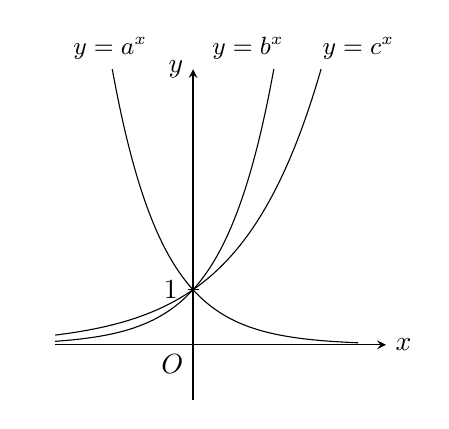
\begin{tikzpicture}[>=stealth, scale=0.7]
            \draw[->] (-2.5,0) --(3.5,0) node[right]{$x$};
            \draw[->] (0,-1) --(0,5) node[left]{$y$};
            \draw (0,0)--(0,0) node[below left]{$O$};
            \draw (-0.1,1)node[left]{$1$}--(0.1,1);
            \begin{scope}
                \clip (-3,-1) rectangle (3.5,5);
                \draw[samples=200,domain=-1.5:3,smooth,variable=\x] plot (\x,{(1/3)^(\x)});
                \draw[samples=200,domain=-2.5:2.5,smooth,variable=\x] plot (\x,{(2)^(\x)});
                \draw[samples=200,domain=-2.5:1.5,smooth,variable=\x] plot (\x,{(3)^(\x)});
            \end{scope}
            \draw (-1.5,5) node[above]{\small $y=a^x$};
            \draw (1,5) node[above]{\small $y=b^x$};
            \draw (3,5) node[above]{\small $y=c^x$};
    \end{tikzpicture}}
    \loigiai{
        \immini{Đường thẳng $x=1$ đồ thị các hàm số $y=a^x$, $y=b^x$, $y=c^x$ tại các điểm có tung độ lần lượt là $y=a$, $y=b$, $y=c$ như hình vẽ.\\
            Từ đồ thị kết luận $ a<c<b$.}
        {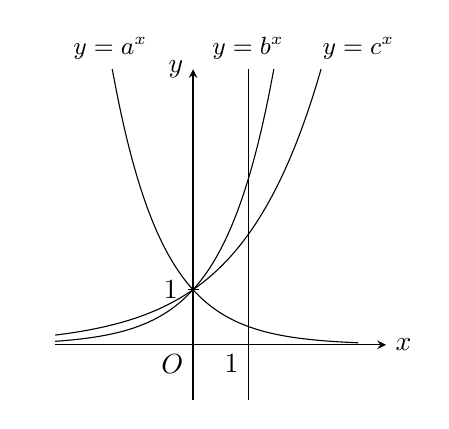
\begin{tikzpicture}[>=stealth, scale=0.7]
                \draw[->] (-2.5,0) --(3.5,0) node[right]{$x$};
                \draw[->] (0,-1) --(0,5) node[left]{$y$};
                \draw (0,0)--(0,0) node[below left]{$O$};
                \draw (-0.1,1)node[left]{$1$}--(0.1,1);
                \begin{scope}
                    \clip (-3,-1) rectangle (3.5,5);
                    \draw[samples=200,domain=-1.5:3,smooth,variable=\x] plot (\x,{(1/3)^(\x)});
                    \draw[samples=200,domain=-2.5:2.5,smooth,variable=\x] plot (\x,{(2)^(\x)});
                    \draw[samples=200,domain=-2.5:1.5,smooth,variable=\x] plot (\x,{(3)^(\x)});
                \end{scope}
                \draw (-1.5,5) node[above]{\small $y=a^x$};
                \draw (1,5) node[above]{\small $y=b^x$};
                \draw (3,5) node[above]{\small $y=c^x$};
                \draw (1,-1)--(1,5);
                \draw (1,0) node[below left]{$1$};
        \end{tikzpicture}}
    }
\end{ex}

\begin{ex}%[2D2B4-3]
    [Mã 105 2017]%Câu 57
    \immini{Cho hàm số $y=a^x$, $y=b^x$ với $ a,b$ là hai số thực dương khác $1$, lần lượt có đồ thị là $\left(C_1\right)$ và $\left(C_2\right)$ như hình bên. Mệnh đề nào dưới đây đúng?
        \choice
        {\True $0<b<1<a$}
        {$0<a<b<1$}
        {$0<b<a<1$}
        {$0<a<1<b$}}
    {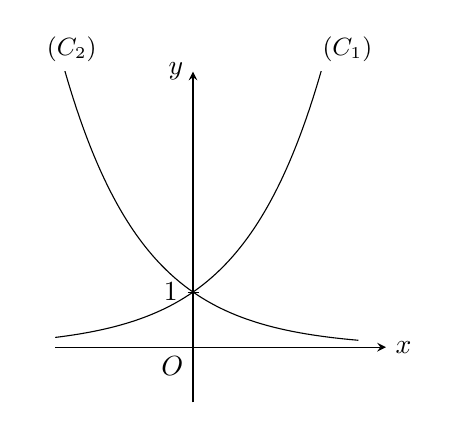
\begin{tikzpicture}[>=stealth, scale=0.7]
            \draw[->] (-2.5,0) --(3.5,0) node[right]{$x$};
            \draw[->] (0,-1) --(0,5) node[left]{$y$};
            \draw (0,0)--(0,0) node[below left]{$O$};
            \draw (-0.1,1)node[left]{$1$}--(0.1,1);
            \begin{scope}
                \clip (-3,-1) rectangle (3.5,5);
                \draw[samples=200,domain=-2.5:3,smooth,variable=\x] plot (\x,{(1/2)^(\x)});
                \draw[samples=200,domain=-2.5:2.5,smooth,variable=\x] plot (\x,{(2)^(\x)});
            \end{scope}
            \draw (-2.2,5) node[above]{\small $(C_2)$};
            \draw (2.8,5) node[above]{\small $(C_1)$};
        \end{tikzpicture}
    }
    \loigiai{
        Theo hình ta thấy hàm $y=a^x$ là hàm đồng biến nên $a>1$, còn hàm $y=b^x$ là hàm nghịch biến nên $0<b<1$. Suy ra $0<b<1<a$.
    }
\end{ex}

\begin{ex}%[2D2B4-3]
    [Chuyên Bắc Giang 2019]%Câu 58
    Trong các hàm số sau hàm số nào nghịch biến trên $\mathbb{R}$?
    \choice
    {$\log_3x^2$}
    {$y=\log\left(x^3\right)$}
    {\True $y=\left(\dfrac{{e}}{4}\right)^x$}
    {$y=\left(\dfrac{2}{5}\right)^{-x}$}
    \loigiai{
        Hàm số mũ $y=a^x$ với $0<a<1$ nghịch biến trên $\mathbb{R}$.\\
        Ta có $0<\dfrac{{e}}{4}<1$ nên hàm số $y=\left(\dfrac{{e}}{4}\right)^x$nghịch biến trên $\mathbb{R}$.
    }
\end{ex}

\begin{ex}%[2D2B4-3]
    Mệnh đề nào trong các mệnh đề dưới đây sai?
    \choice
    {Hàm số $y=\left(\dfrac{2018}{\pi}\right)^{x^2+1}$ đồng biến trên $\mathbb{R}$}
    {Hàm số $y=\log x$ đồng biến trên $\left(0;+\infty\right)$}
    {\True Hàm số $y=\ln\left(-x\right)$ nghịch biến trên khoảng $\left(-\infty;0\right)$}
    {Hàm số $y=2^x$ đồng biến trên $\mathbb{R}$}
    \loigiai{
        Hàm số $y=\ln(-x)$. Tập xác định $\mathscr{D}=\left(-\infty;0\right)$.\\
        Cơ số $a=e>1$. Do đó hàm số đồng biết trên $\left(-\infty;0\right)$.
    }
\end{ex}

\begin{ex}%[2D2B4-3]
    [THPT An Lão Hải Phòng 2019]%Câu 60
    Hàm số nào dưới đây đồng biến trên tập xác định của nó?
    \choice
    {$y=\left(\dfrac{1}{\pi}\right)^x$}
    {$y=\left(\dfrac{2}{3}\right)^x$}
    {\True $y=\left(\sqrt{3}\right)^x$}
    {$y=\left(0,5\right)^x$}
    \loigiai{
        Hàm số $y=a^x$ đồng biến trên $\mathbb{R}$ khi và chỉ khi $a>1$.\\
        Thấy các số $\dfrac{1}{\pi};\dfrac{2}{3};0,5$ nhỏ hơn $1$, còn $\sqrt{3}$ lớn hơn $1$ nên chọn C.
    }
\end{ex}

\begin{ex}%[2D2B4-3]
    [THPT An Lão Hải Phòng 2019]%Câu 61
    Cho hàm số $y=\log_2x$. Mệnh đề nào dưới đây sai?
    \choice
    {Đạo hàm của hàm số là $y'=\dfrac{1}{x\ln 2}$}
    {Đồ thị hàm số nhận trục $Oy$ làm tiệm cận đứng}
    {\True Tập xác định của hàm số là $\left(-\infty;+\infty\right)$}
    {Hàm số đồng biến trên khoảng $\left(0;+\infty\right)$}
    \loigiai{
        Hàm số $y=\log_2x$ có tập xác định là $\mathscr{D}=\left(0;+\infty\right)$.
    }
\end{ex}

\begin{ex}%[2D2B4-3]
    [THPT Lê Quy Đôn Điện Biên 2019]%Câu 62
    Trong các hàm số sau, hàm số nào luôn đồng biến trên $\mathbb{R}$?
    \choice
    {$y=\left(\dfrac{2015}{2016}\right)^x$}
    {$y=\left(\dfrac{3}{\sqrt{2016}-\sqrt{2}}\right)^x$}
    {$y=(0,1) ^{2x}$}
    {\True $y=(2016)^{2 x}$}
    \loigiai{
        ${y}=(0,1)^{2x}=\left(0,01\right)^x$, $y=(2016)^{2x}=4064256^x$.\\
        Ta có các cơ số $\dfrac{2015}{2016}$; $\dfrac{3}{\sqrt{2016}-\sqrt{2}}$; $ 0,01$ đều nhỏ hơn $1$ nên các hàm số ở A, B, C nghịch biến trên $\mathbb{R}$.\\
        Cơ số $4064256>1$ nên hàm số $y=(2016) ^{2 x}$ đồng biến trên $\mathbb{R}$.
    }
\end{ex}

\begin{ex}%[2D2B4-3]
    \immini{Đường cong trong hình vẽ bên là đồ thị của hàm số nào dưới đây?
        \choice
        {$y=-{\mathrm{e}}^x$}
        {$y=\left|\ln x\right|$}
        {\True $y=\ln x$}
        {$y={\mathrm{e}}^x$}}
    {\begin{tikzpicture}[>=stealth,scale=0.9, line join=round, line cap=round]
            \def\xp{3.5} \def\yt{3} \def\yd{-2.2}
            \draw[->] (-0.9,0)--(\xp,0) node [below]{$x$};
            \draw[->] (0,\yd)--(0,\yt) node [left]{$y$};
            \node at (0,0) [below left]{$O$};
            \foreach \p/\r in {1/-90,2/-90}
            \fill (\p,0) circle (1pt) node[shift={(\r:3mm)}]{$\p$};
            \foreach \p/\r in {1/180,2/180}
            \fill (0,\p) circle (1pt) node[shift={(\r:3mm)}]{$\p$};
            \draw[dashed] (e,0) node[below] {$\mathrm{e}$} -- (e,1)--(0,1);
            \clip (-0.9,\yd) rectangle (\xp-0.1,\yt-0.1);
            \draw[smooth,samples=300,domain=0.03:\xp] plot(\x,{ln(\x)});
        \end{tikzpicture}
    }
    \loigiai{
        Đồ thị hàm số đi qua điểm $\left(\mathrm{e}; 1\right)$ và nằm cả trên và dưới trục hoành nên chỉ có hàm số $y=\ln x$ thoả mãn.
    }
\end{ex}

\begin{ex}%[2D2B4-3]
    [Chuyên Lê Thánh Tông 2019]%Câu 64
    Hàm số nào sau đây đồng biến trên $\mathbb{R}$.
    \choice
    {\True $f(x)=3^x$}
    {$f(x)=3^{-x}$}
    {$f(x)=\left(\dfrac{1}{\sqrt{3}}\right)^x$}
    {$f(x)=\dfrac{3}{3^x}$}
    \loigiai{
        Hàm số $f(x)=a^x$ đồng biến trên $\mathbb{R}$ nếu $ a>1$ và nghịch biến trên $\mathbb{R}$ nếu $ 0<a<1$.\\
        Vậy hàm số $ f(x)=3^x$ là hàm số đồng biến trên $\mathbb{R}$.
    }
\end{ex}

\begin{ex}%[2D2B4-3]
    [Chuyên Bắc Ninh 2019]%Câu 65
    Cho hàm số $y=\log_{\sqrt{5}}x$. Mệnh đề nào dưới đây là mệnh đề sai?
    \choice
    {Hàm số đã cho đồng biến trên tập xác định}
    {\True Hàm số đã cho có tập xác định $\mathscr{D}=\mathbb{R}\backslash\left\{0\right\}$}
    {Đồ thị hàm số đã cho có một tiệm cận đứng là trục tung}
    {Đồ thị hàm số đã cho không có tiệm cận ngang}
    \loigiai{
        Ta có tập xác định của hàm số $y=\log_{\sqrt{5}}x$ là $\mathscr{D}=\left(0;+\infty\right)$. Do đó đáp án B sai.
    }
\end{ex}

\begin{ex}%[2D2B4-3]
    \immini{Cho đồ thị hàm số $y=a^x$ và $y=\log_bx$ như hình vẽ.
        Khẳng định nào sau đây đúng?
        \choice
        {$0<a<\dfrac{1}{2}<b$}
        {\True $0<a<1<b$}
        {$0<b<1<a$}
        {$0<a<1$, $0<b<\dfrac{1}{2}$}}
    {\begin{tikzpicture}[>=stealth,scale=0.9, line join=round, line cap=round]
            \def\xp{3.5} \def\yt{3} \def\yd{-2.2}
            \draw[->] (-2.5,0)--(\xp,0) node [below]{$x$};
            \draw[->] (0,\yd)--(0,\yt) node [left]{$y$};
            \node at (0,0) [below left]{$O$};
            \foreach \p/\r in {1/-90}
            \fill (\p,0) circle (1pt) node[shift={(\r:3mm)}]{$\p$};
            \foreach \p/\r in {1/180}
            \fill (0,\p) circle (1pt) node[shift={(\r:3mm)}]{$\p$};
            \begin{scope}
                \clip (-2.5,-2.2) rectangle (3.5,3);
                \draw[smooth,samples=300,domain=0.03:\xp] plot(\x,{ln(\x)});
                \draw[samples=200,domain=-2:3,smooth,variable=\x] plot (\x,{(2/3)^(\x)});
            \end{scope}
    \end{tikzpicture}}
    \loigiai{
        Xét hàm số $y=a^x$ đi qua $\left(0;1\right)$ suy ra đồ thị hàm số $(1)$ là đồ thị của hàm nghịch biến nên $0<a<1$.\\
        Xét đồ thị hàm số $y=\log_bx$ đi qua $\left(1;0\right)$ suy ra đồ thị của hàm số $(2)$ là đồ thị của hàm đồng biến suy ra $b>1$.\\
        Vậy $0<a<1<b$.
    }
\end{ex}

\begin{ex}%[2D2B4-3]
    [Chuyên Lê Quý Đôn Điện Biên 2019]%Câu 67
    Trong các hàm số sau, hàm số nào nghịch biến?
    \choice
    {$y=\ln x$}
    {$y=\log_{1-\sqrt{\frac{2018}{2019}}}x$}
    {$y=\log_{\pi}x$}
    {\True $y=\log_{4-\sqrt{3}}x$}
    \loigiai{
        Xét hàm số $y=\ln x$.\\
        TXĐ $\mathscr{D}=\left(0;+\infty\right)$\\
        $e>1$ suy ra hàm số $y=\ln x$ đồng biến trên $\mathscr{D}$.\\
        Xét hàm số $y=\log_{1-\sqrt{\frac{2018}{2019}}}x$.\\
        TXĐ $\mathscr{D}=\left(0;+\infty\right)$\\
        $0<\sqrt{\dfrac{2018}{2019}}<1\Rightarrow 0<1-\sqrt{\dfrac{2018}{2019}}<1$ suy ra hàm số $y=\log_{1-\sqrt{\frac{2018}{2019}}}x$ là hàm nghịch biến\\
        $\mathscr{D}$.\\
        Xét hàm số $y=\log_{\pi}x$. \\
        TXĐ $\mathscr{D}=\left(0;+\infty\right)$\\
        $\pi >1$ suy ra hàm số $y=\log_{\pi}x$ đồng biến trên $\mathscr{D}$.\\
        Xét hàm số $y=\log_{4-\sqrt{3}}x$.\\
        TXĐ $\mathscr{D}=\left(0;+\infty\right)$\\
        $4-\sqrt{3}>1$ suy ra hàm số $y=\log_{4-\sqrt{3}}x$ đồng biến trên $\mathscr{D}$.
    }
\end{ex}

\begin{ex}%[2D2B4-3]
    [Sở Hà Nội 2019]%Câu 68
    Đồ thị hàm số $y=\ln x$ đi qua điểm
    \choice
    {\True $\left(1;0\right)$}
    {$\left(2;{\mathrm{e}^2}\right)$}
    {$\left(2\mathrm{e};2\right)$}
    {$\left(0;1\right)$}
    \loigiai{
        Với $x=1\Rightarrow y=\ln 1=0$.\\
        Với $x=2\Rightarrow y=\ln 2$.\\
        Với $x=2\mathrm{e}\Rightarrow y=\ln 2\mathrm{e}=\ln 2+1$.\\
        Với $x=0$, hàm số không xác định.
    }
\end{ex}

\begin{ex}%[2D2B4-3]
    [Chuyên Lương Thế Vinh Đồng Nai 2019]%Câu 69
    Trong các hàm số sau,hàm số nào luôn nghịch biến trên tập xác định của nó?
    \choice
    {$y=\left(\dfrac{1}{2}\right)^2$}
    {$y=\log x$}
    {$y=2^x$}
    {\True $y=\left(\dfrac{2}{3}\right)^x$}
    \loigiai{
        Ta thấy hàm số $y=\left(\dfrac{2}{3}\right)^x$là hàm số mũ có có tập xác định là $\mathbb{R}$ cơ số $a=\dfrac{2}{3}<1$ nên nghịch biến trên tập xác định của nó.\\
        Ngoài ra ta có thể loại các đáp án khác bằng cách giải thích cụ thể đặc điểm các hàm đó như sau:\\
        Đáp án A loại vì Hàm số $y=\left(\dfrac{1}{2}\right)^2$ là hàm hằng nên không nghịch biến cũng không đồng biến.\\
        Đáp án B loại vì Hàm số $y=\log x$ là hàm số logarit có tập xác định là $\mathscr{D}=(0;+\infty)$ có cơ số $a=10>1$ nên luôn đồng biến trên tập xác định của nó.\\
        Đáp án C loại vì hàm số $y=2^x$ là hàm số mũ có tập xác định là $\mathbb{R}$có cơ số $a=2>1$.
    }
\end{ex}

\begin{ex}%[2D2B4-3]
    [Chuyên Lương Thế Vinh Đồng Nai 2019]%Câu 70
    Chọn khẳng định sai trong các khẳng định sau
    \choice
    {\True Hàm số $y=\log_2x$ đồng biến trên $\mathbb{R}$}
    {Hàm số $y=\log_{\frac{1}{2}}x$ nghịch biến trên tập xác định của nó}
    {Hàm số $y=2^x$ đồng biến trên $\mathbb{R}$}
    {Hàm số $y=x^{\sqrt{2}}$ có tập xác định là $\left(0;+\infty\right)$}
    \loigiai{
        Hàm số $y=\log_2x$ đồng biến trên khoảng $\left(0;+\infty\right)$.
    }
\end{ex}

\begin{ex}%[2D2B4-3]
    [KTNL GV Bắc Giang 2019]%Câu 71
    Hàm số nào dưới đây đồng biến trên khoảng $(0;+\infty)$?
    \choice
    {\True $y=\log_{\sqrt{3}}x$}
    {$y=\log_{\frac{\pi}{6}}x$}
    {$y=\log_{\frac{e}{3}}x$}
    {$y=\log_{\frac{1}{4}}x$}
    \loigiai{
        Hàm số $y=\log_ax$ đồng biến trên khoảng $(0;+\infty)\Leftrightarrow a>1\Rightarrow$ chọn A.
    }
\end{ex}

\begin{ex}%[2D2B4-3]
    [Chuyên Lê Hồng Phong Nam Định 2019]%Câu 72
    Trong các mệnh đề sau, mệnh đề nào đúng?
    \choice
    {Đồ thị của hàm số $y=2^x$ và $y=\log_2x$ đối xứng với nhau qua đường thẳng $y=-x$}
    {\True Đồ thị của hai hàm số $y=\mathrm{e}^x$ và $y=\ln x$ đối xứng với nhau qua đường thẳng $y=x$}
    {Đồ thị của hai hàm số $y=2^x$ và hàm số $y=\dfrac{1}{2^x}$ đối xứng với nhau qua trục hoành}
    {Đồ thị của hai hàm số $y=\log_2x$ và $y=\log_2\dfrac{1}{x}$ đối xứng với nhau qua trục tung}
    \loigiai{
        Đồ thị hàm số $y=a^x$ và đồ thị hàm số $y=\log_ax$ đối xứng với nhau qua đường phân giác góc\\
        phần tư thứ nhất ($y=x$), suy ra chọn B.
    }
\end{ex}

\begin{ex}%[2D2B4-3]
    [Chuyên Lê Hồng Phong Nam Định 2019]%Câu 73
    \immini{Hàm số nào sau đây có đồ thị như hình bên?
        \choice
        {$y=\log_3x$}
        {$y=\log_2x+1$}
        {\True $y=\log_2\left(x+1\right)$}
        {$y=\log_3\left(x+1\right)$}}
    {\begin{tikzpicture}[>=stealth,scale=0.9, line join=round, line cap=round]
            \draw[->] (-2,0)--(3,0) node [below]{$x$};
            \draw[->] (0,-2)--(0,3) node [left]{$y$};
            \node at (0,0) [below left]{$O$};
            \foreach \p/\r in {1/-90,2/-90,-1/-145}
            \fill (\p,0) circle (1pt) node[shift={(\r:3mm)}]{$\p$};
            \foreach \p/\r in {1/180,2/180}
            \fill (0,\p) circle (1pt) node[shift={(\r:3mm)}]{$\p$};
            \draw (-1,-2)--(-1,3);
            \draw[dashed] (0,1)--(1,1)--(1,0);
            \begin{scope}
                \clip (-2,-2) rectangle (3,3);
                \draw[smooth,samples=300,domain=-0.8:3] plot(\x,{ln((\x)+1)/ln(2)});
            \end{scope}
    \end{tikzpicture}}
    \loigiai{
        Đồ thị hàm số đi qua điểm $\left(0;0\right)$ nên loại đáp án A và B.\\
        Đồ thị hàm số đi qua điểm $\left(1;1\right)$ nên loại D.\\
        Vậy đáp án C thỏa mãn.
    }
\end{ex}

\begin{ex}%[2D2B4-3]
    [Chuyên Quốc Học Huế 2019]%Câu 74
    Trong các hàm số dưới đây, hàm số nào nghịch biến trên tập số thực $\mathbb{R}$.
    \choice
    {$y=\left(\dfrac{\pi}{3}\right)^x$}
    {$y=\log_{\frac{\pi}{4}}\left(2x^2+1\right)$}
    {\True $y=\left(\dfrac{2}{\mathrm{e}}\right)^x$}
    {$y=\log_{\frac{2}{3}}x$}
    \loigiai{
        Vì $\dfrac{2}{\mathrm{e}}<1$ nên $y=\left(\dfrac{2}{e}\right)^x$nghịch biến trên $\mathbb{R}$.
    }
\end{ex}

\begin{ex}%[2D2B4-3]
    [Chuyên Vĩnh Phúc 2019]%Câu 75
    Hàm số nào dưới đây nghịch biến trên tập xác định của nó?
    \choice
    {$y=\log_{\sqrt{3}}x$}
    {$y=\log_2\left(\sqrt{x}+1\right)$}
    {\True $y=\log_{\frac{\pi}{4}}x$}
    {$y=\left(\dfrac{\pi}{3}\right)^x$}
    \loigiai{
        Xét hàm số $ y=\log_{\frac{\pi}{4}}x$ có tập xác định: $\mathscr{D}=\left(0;+\infty\right)$.\\
        Nhận thấy cơ số $\dfrac{\pi}{4}<1$ nên $ y=\log_{\frac{\pi}{4}}x$ nghịch biến trên tập xác định.
    }
\end{ex}

\begin{ex}%[2D2B4-3]
    [Chuyên Bắc Giang - 2019]%Câu 76
    Cho hàm số $y=\dfrac{3^x}{\ln 3}-9x+17$. Mệnh đề nào sau đây sai?
    \choice
    {Hàm số nghịch biến trên khoảng $\left(-\infty;0\right)$}
    {\True Hàm số đồng biến trên khoảng $\left(0;+\infty\right)$}
    {Hàm số đạt cực trị tại $x=2$}
    {Hàm số có giá trị cực tiểu là $y=\dfrac{9}{\ln 3}-1$}
    \loigiai{
        Ta có $y'=\dfrac{3^x\ln 3}{\ln 3}-9=3^x-9$\\
        $ y'=0\Leftrightarrow{3^x}=9\Leftrightarrow x=2$
        \begin{center}
            
\begin{tikzpicture}
                \tkzTabInit[nocadre,lgt=1,espcl=3]{$x$/0.8,$y'$/0.8,$y$/2.5}{$-\infty$,$2$,$+\infty$}
                \tkzTabLine{,-,0,+,}
                \tkzTabVar{+/{},-/$\dfrac{9}{\ln3}-1$,+/{}}
            \end{tikzpicture}
        \end{center}
    }
\end{ex}

\begin{ex}%[2D2B4-3]
    [THPT Lê Quy Đôn Điện Biên - 2019]%Câu 77
    Đồ thị $(L)$ của hàm số $f(x)=\ln x$ cắt trục hoành tại điểm $A$, tiếp tuyến của $(L)$ tại $A$ có phương trình là
    \choice
    {$y=2x+1$}
    {\True $y=x-1$}
    {$y=3x$}
    {$y=4x-3$}
    \loigiai{
        TXĐ $\mathscr{D}=\left(0;+\infty\right)$. $f'(x)=\dfrac{1}{x}$\\
        Xét phương trình hoành độ giao điểm $\ln x=0\Leftrightarrow x=1\Rightarrow A\left(1;0\right)$\\
        Vậy phương trình tiếp tuyến của đồ thị hàm số $(L)$ tại điểm $A$ là\\
        $ y=f'(1)\left(x-1\right)+0=x-1$, chọn B.
    }
\end{ex}

\begin{ex}%[2D2B4-3]
    [THCS - THPT Nguyễn Khuyến 2019]%Câu 78
    Hàm số $y=x{\mathrm{e}^{-3x}}$ đạt cực đại tại
    \choice
    {$x=\dfrac{1}{3\mathrm{e}}$}
    {\True $x=\dfrac{1}{3}$}
    {$x=\dfrac{1}{\mathrm{e}}$}
    {$x=0$}
    \loigiai{
        Tập xác định là $\mathbb{R}$.\\
        $y'=\mathrm{e}^{-3x}\left(1-3x\right)$.\\
        Vì $\mathrm{e}^{-3x}>0$, $\forall x\in\mathbb{R}$ nên dấu của $y'$ là dấu của nhị thức $1-3x$, suy ra $y'$ đổi dấu từ dương sang âm khi $x$ đi qua $\dfrac{1}{3}$.\\
        Do đó, $ x=\dfrac{1}{3}$ là điểm cực đại của hàm số.
    }
\end{ex}

\begin{ex}%[2D2B4-3]
    [THPT Gia Lộc Hải Dương 2019]%Câu 79
    Hàm số $y=\log_3\left(x^2-2x\right)$ nghịch biến trên khoảng nào?
    \choice
    {$\left(2;+\infty\right)$}
    {\True $\left(-\infty;0\right)$}
    {$\left(1;+\infty\right)$}
    {$\left(0;1\right)$}
    \loigiai{
        Hàm số $y=\log_3\left(x^2-2x\right)$ có tập xác định $\mathscr{D}=\left(-\infty;0\right)\cup\left(2;+\infty\right)$.\\
        Ta có $y'=\dfrac{2x-2}{\left(x^2-2x\right)\ln 3}$. Khi đó $y'=0$ $\Leftrightarrow x=1$.\\
        Bảng biến thiên
        \begin{center}
            \begin{tikzpicture}[yscale=1,xscale=1.5]
                \def\c{7}%số cột
                \def\d{4}%số dòng
                \foreach \x in {0,...,\c}{
                    \foreach \y in {0,...,\d}
                    \path[yscale=-1] (\x,\y) node[gray!0,minimum size=1cm] (\x\y) {\x\y};
                }
                \draw[shift={(-0.5,0.5)}]
                %(0,0) rectangle (\c+1,-\d-1)
                (0,-1)--(\c+1,-1)
                (0,-2)--(\c+1,-2)
                (1,0)--(1,-\d-1);
                \path
                (00) node {$x$}
                (10) node {$-\infty$}
                (30) node {$0$}
                (50) node {$2$}
                (70) node {$+\infty$}
                (01) node {$y'$}
                (21) node {$-$}
                (61) node {$+$}
                (03) node {$y$}
                (12) node {$+\infty$}
                (34) node[left] {$-\infty$}
                (54) node[right] {$-\infty$}
                (72) node {$+\infty$}
                ;
                \fill[pattern=north east lines] (34.south) rectangle ([shift={(0,-0.2mm)}]51.north);
                \draw[double distance=2pt]([shift={(0,-0.2mm)}]31.north)--(34.south);
                \draw[double distance=2pt]([shift={(0,-0.2mm)}]51.north)--(54.south);
                \foreach \a/\b in {12/34,54/72}
                \draw[->,>=stealth] (\a)--(\b);
            \end{tikzpicture}
        \end{center}
        Dựa vào bảng biến thiên ta có hàm số $y$ nghịch biến trên $\left(-\infty;0\right)$.
    }
\end{ex}

\begin{ex}%[2D2B4-3]
    \immini{Cho đồ thị hàm số $y=a^x$ và $y=\log_bx$ như hình vẽ. Trong các khẳng định sau, đâu là khẳng định đúng.
        \choice
        {$0<a<1$, $0<b<1$}
        {$a>1$, $b>1$}
        {\True $0<b<1<a$}
        {$0<a<1<b$}}
    {\begin{tikzpicture}[>=stealth,scale=0.9, line join=round, line cap=round]
            \def\xp{3.5} \def\yt{3} \def\yd{-1.5}
            \draw[->] (-2.5,0)--(\xp,0) node [below]{$x$};
            \draw[->] (0,\yd)--(0,\yt) node [left]{$y$};
            \node at (0,0) [below left]{$O$};
            \foreach \p/\r in {1/-90}
            \fill (\p,0) circle (1pt) node[shift={(\r:3mm)}]{$\p$};
            \foreach \p/\r in {1/180}
            \fill (0,\p) circle (1pt) node[shift={(\r:3mm)}]{$\p$};
            \begin{scope}
                \clip (-2.5,-1.5) rectangle (3.5,3);
                \draw[smooth,samples=300,domain=0.03:\xp] plot(\x,{ln(\x)/ln(0.5)});
                \draw[samples=200,domain=-2.5:3,smooth,variable=\x] plot (\x,{(2)^(\x)});
            \end{scope}
    \end{tikzpicture}}
    \loigiai{
        Dựa vào đồ thị ta thấy khi $x\to-\infty\Rightarrow y\Rightarrow 0$ do đó đồ thị hàm số $y=a^x$ có $a>1$. Nên ta loại đáp án A và D.\\
        Ở đồ thị hàm số $y=\log_bx\Leftrightarrow x=b^y$ ta thấy khi $x\to+\infty\Rightarrow y\Rightarrow-\infty$ do đó ta có $0<b<1$.
    }
\end{ex}

\begin{ex}%[2D2B4-3]
    \immini{Hình vẽ bên thể hiện đồ thị của ba trong bốn hàm số $y=6^x$, $y=8^x$, $y=\dfrac{1}{5^x}$ và $ y=\dfrac{1}{\sqrt{7}^x}$.
        Hỏi $(C_2)$ là đồ thị hàm số nào?
        \choice
        {$y=6^x$}
        {$y=\dfrac{1}{\sqrt{7}^x}$}
        {\True $y=\dfrac{1}{5^x}$}
        {$y=8^x$}}
    {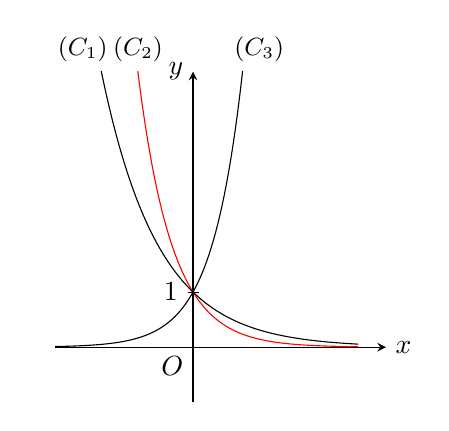
\begin{tikzpicture}[>=stealth, scale=0.7]
            \draw[->] (-2.5,0) --(3.5,0) node[right]{$x$};
            \draw[->] (0,-1) --(0,5) node[left]{$y$};
            \draw (0,0)--(0,0) node[below left]{$O$};
            \draw (-0.1,1)node[left]{$1$}--(0.1,1);
            \begin{scope}
                \clip (-3,-1) rectangle (3.5,5);
                \draw[red,samples=200,domain=-1.5:3,smooth,variable=\x] plot (\x,{(1/5)^(\x)});
                \draw[samples=200,domain=-2.5:2.5,smooth,variable=\x] plot (\x,{(6)^(\x)});
                \draw[samples=200,domain=-2.5:3,smooth,variable=\x] plot (\x,{(0.38)^(\x)});
            \end{scope}
            \draw (-2,5) node[above]{\small $(C_1)$};
            \draw (-1,5) node[above]{\small $(C_2)$};
            \draw (1.2,5) node[above]{\small $(C_3)$};
    \end{tikzpicture}}
    \loigiai{
        Hàm số có đồ thị $(C_2)$ là hàm số nghịch biến, do đó loại đáp án A, D. Cho $x=1$ suy ra $\dfrac{1}{\sqrt{7}}>\dfrac{1}{5}$\\
        Do đó đồ thị hàm số $(C_2)$ là $y=\dfrac{1}{5^x}$.
    }
\end{ex}

\begin{ex}%[2D2B4-3]
    [Chuyên Lê Hồng Phong Nam Định 2019]%Câu 82
    Giá trị nhỏ nhất của hàm số $y=\dfrac{\ln x}{x}$ trên đoạn $\left[2;3\right]$ bằng
    \choice
    {\True $\dfrac{\ln 2}{2}$}
    {$\dfrac{\ln 3}{3}$}
    {$\dfrac{3}{\mathrm{e}^2}$}
    {$\dfrac{1}{\mathrm{e}}$}
    \loigiai{
        Xét $y=f(x)=\dfrac{\ln x}{x}$. Hàm số $y=f(x)$ liên tục trên đoạn $\left[2;3\right]$\\
        $y'=\dfrac{1-\ln x}{x^2}$; $y'=0$ $\Leftrightarrow\dfrac{1-\ln x}{x^2}=0$ $\Leftrightarrow x=e\in\left[2;3\right]$\\
        Có $f(2)=\dfrac{\ln 2}{2}\approx 0,3466$; $f(\mathrm{e})=\dfrac{1}{\mathrm{e}}\approx 0,3679$; $f(3)=\dfrac{\ln 3}{3}\approx 0,366$.\\
        Suy ra $\underset{x\in\left[2;3\right]}{\min}f(x)=\dfrac{\ln 2}{2}$.\\
        Vậy giá trị nhỏ nhất của hàm số $y=\dfrac{\ln x}{x}$ trên đoạn $\left[2;3\right]$ bằng $\dfrac{\ln 2}{2}$.
    }
\end{ex}

\begin{ex}%[2D2B4-3]
    [Sở Ninh Bình 2019]%Câu 83
    Cho hàm số $f(x)=\ln x-x$. Khẳng định nào dưới đây đúng?
    \choice
    {\True Hàm số đồng biến trên khoảng $\left(0;1\right)$}
    {Hàm số đồng biến trên khoảng $\left(0;+\infty\right)$}
    {Hàm số đồng biến trên các khoảng $\left(-\infty ;0\right)$ và $\left(1;+\infty\right)$}
    {Hàm số đồng biến trên khoảng $\left(1;+\infty\right)$}
    \loigiai{
        Tập xác định của hàm số $ f(x)$ $\mathscr{D}=\left(0;+\infty\right)$.\\
        Ta có $f'(x)=\dfrac{1}{x}-1=\dfrac{1-x}{x}$.\\
        $f'(x)=0\Rightarrow x=1$.\\
        Bảng xét dấu $f'(x)$
        \begin{center}
            
\begin{tikzpicture}
                \tkzTabInit[nocadre,lgt=1.2,espcl=2]{$x$/0.8,$f'(x)$/0.8}{$0$,$1$,$+\infty$}
                \tkzTabLine{,+,0,-,}
            \end{tikzpicture}
        \end{center}
        Vậy hàm số đã cho đồng biến trên khoảng $\left(0;1\right)$ và nghịch biến trên khoảng $\left(1;+\infty\right)$.
    }
\end{ex}

\begin{ex}%[2D2B4-3]
    [HSG Bắc Ninh 2019]%Câu 84
    Giá trị nhỏ nhất của hàm số $f(x)=\left(x^2-2\right){\mathrm{e}^{2x}}$ trên đoạn $\left[-1;2\right]$ bằng
    \choice
    {$2\mathrm{e}^4$}
    {\True $-\mathrm{e}^2$}
    {$2\mathrm{e}^2$}
    {$-2\mathrm{e}^2$}
    \loigiai{
        Ta có $f'(x)=2\left(x^2-2\right){\mathrm{e}^{2x}}+2x{\mathrm{e}^{2x}}=2\left(x^2+x-2\right){\mathrm{e}^{2x}}$.\\
        $f'(x)=0\Leftrightarrow\left[\begin{aligned}
            &x=1\in\left[-1;2\right]\\
            &x=-2\notin\left[-1;2\right]\\
        \end{aligned}\right.$.\\
        Và $f\left(-1\right)=-\mathrm{e}^{-2}$; $f(2)=2\mathrm{e}^4$; $f(1)=-\mathrm{e}^2$.\\
        Giá trị nhỏ nhất của hàm số $f(x)=\left(x^2-2\right){\mathrm{e}^{2x}}$ trên đoạn $\left[-1;2\right]$ bằng $-\mathrm{e}^2$ tại $x=1$.
    }
\end{ex}

\begin{ex}%Câu 85%[2D2B4-3]
    Giá trị nhỏ nhất của hàm số $y=2^{x+1}-\dfrac{4}{3}\cdot{8^x}$ trên $\left[-1;0\right]$ bằng
    \choice
    {$\dfrac{4}{9}$}
    {$\dfrac{5}{6}$}
    {$\dfrac{2\sqrt{2}}{3}$}
    {\True $\dfrac{2}{3}$}
    \loigiai{
        $y'=2^{x+1}\ln 2-\dfrac{4}{3}\cdot{8^x}\ln 8=0\Leftrightarrow{2^x}-2\cdot{\left(2^x\right)^3}=0\Leftrightarrow\left[\begin{aligned}
            &{2^x}=0\\
            &{2^x}=\dfrac{1}{\sqrt{2}}\\
        \end{aligned}\right.\Leftrightarrow\left[\begin{aligned}
            &x=1\\
            &x=-\dfrac{1}{2}.\\
        \end{aligned}\right.$\\
        Xét $y(-1)=\dfrac{5}{6}$; $y(-\dfrac{-1}{2})=0,9428$; $y(0)=\dfrac{2}{3}$. Ta có $y_{\min}=\dfrac{2}{3}$.
    }
\end{ex}

\Closesolutionfile{ans}
\indapan{10}{ans/CD18/Muc_5_6}